\chapter{Interface descriptionToBeDel}
\label{Chapter4}
\section{Introduction to watermarking}
%This section outline the general digital image watermarking elements and their operations 
Digital watermarking is a method of inducing secured secret message (watermark) on the digital image (cover image) providing secrecy of the information being transmitted, ownership, authentication, copyright protection \cite{P15} by using suitable algorithm and keys. 

Watermarking can be classified into different categories based on different applications and requirements.

\begin{enumerate}
\item[a)] Based on visibility of watermark :  $i)$ \textit{Visible watermarking} and $ii)$ \textit{Invisible watermarking}. Applications involving to provide identity, ownership, copy right protection makes use of visible watermarking techniques as in currency notes, company logos on the documents. Applications make use of invisible watermarking techniques to provide authentication in transmitting the secret message.
\item[b)] Based on domain of operations : $i)$ \textit{Spatial domain watermarking} and $ii)$ \textit{Frequency domain watermarking}. Amount of robustness and imperceptibility decides the use of these techniques. Least significant bit modification is the simplest example of spatial domain where as DCT, DWT coefficients modifications are some of examples of frequency domain techniques.
\item[c)] Based on level of information required to detect : $i)$ \textit{Blind watermarking} detects the embedded information from the watermarked image without the use of original signal. These blind watermarking techniques are less robust to attacks. These are also called public watermarking technique. $ii)$ \textit{Semi-blind watermarking} detects the embedded information from watermarked image with some knowledge of keying and without using original signal. These are also called semi private watermarking techniques. $iii)$ \textit{Non-blind watermarking} detects the watermark with all the information available at transmission end i.e., original signal and keys. These are also called private watermarking techniques. These techniques are more robust for various attacks compared to other two techniques.
\item[d)] Based on the knowledge of the user on the presence of watermark : $i)$ \textit{Steganographic watermarking} user is not aware of presence of watermark. $ii)$ \textit{Non-steganographic watermarking} user is aware of presence of watermark.
\item[e)] Based on the sensitiveness of the watermark to be destroyed : $i)$ \textit{Fragile watermarking} are very sensitive and destroyed easily by changing little modifications on the watermarked signal. $ii)$ \textit{Semi-fragile watermarking} in which watermarks can be broken if the modifications goes above predetermined thresholds. $iii)$ \textit{Robust watermarking} in which watermarks cannot be destroyed easily as they withstand for different attacks.
\item[f)] Based on authorisation of user to detect watermark : $i)$ \textit{Public watermarking} in which user has authorisation for the detection of embedded watermark in the signal. $ii)$ \textit{Private watermarking} in which user is not authorised to detect the watermark embedded in the signal.
\end{enumerate}	
	

	The most general digital watermarking scheme is shown in Fig \ref{Fig:GWMS}. At transmission end, user specific algorithm is used for embedding the watermark on the original cover image. The watermarked image is transmitted over the noisy channel. Noisy watermarked image is available at the reception end. At reception end, watermark is extracted by using the knowledge of algorithm and keys used at transmission end. The imperceptibility of the watermarked image and robustness of extracted watermark are assessed using the quality assessment metrics such as listed in Section \ref{WMQAP}.\\

 \begin{figure*}
 \centering
 \includegraphics[width=1\linewidth]{./WMSystem2.png}
 \caption{General Watermarking System.}
 \label{Fig:GWMS}
\end{figure*}

Rapid dynamic growth of multimedia technology and evaluation of advanced image processing techniques caters the need for secured watermarking of data. With the evaluation of new technologies, techniques providing authentication, ownership and secrecy of transmission information is a challenging task. Most of the existing techniques of watermarking in the literature are based on either spatial or frequency domain methods \cite{P4}- \cite{P22}. \\

A watermarking method uses DWT, DCT and SVD (W2CS) in which block based DCT is applied on to level-2 HH coefficients of DWT of cover image and singular values are obtained by forming a DC coefficient matrix of the blocks. The singular values thus obtained are modified based on the singular values obtained from watermark and inverse operation of SVD and DWT are applied to get the watermarked image \cite{P4}. Another method makes use of both SWT and SVD (SW1S) techniques in which level-1 decomposition of SWT (Stationery Wavelet Transform) is applied on both cover image and watermark, then SVD is applied on LL coefficients of both cover and watermark. Finally, singular values thus obtained for cover image are modified with the singular values obtained for watermark and inverse operation of SVD and SWT are applied to get watermarked image \cite{P5}. In a DWT and DCT (W1C) approach, block based DCT is applied on to the LL coefficients of level-1 DWT decomposition of cover image. The obtained DCT coefficients in each block are modified based on the watermark and then an inversion is applied before transmitting the watermarked image \cite{P6}. In DWT along with SVD LU decomposition method (W1SLU), LL coefficients of level-1 decomposition of DWT of cover image undergoes LDU decomposition and SVD is applied on to the D coefficients. Then these singular values are modified using the singular values of watermark and inversion is applied over the obtained coefficients for the generation of watermarked image \cite{P7}. Another approach, uses both DCT and DWT (CW3) in which DCT coefficients of watermark are used to modify level-3 DWT HH coefficients \cite{P20}. In, one time pad level-1 DWT method (1PW1) at first a key is generated from the cover image using block divisibility which is used for encrypting the watermark, then level-1 mid frequency DWT coefficients of original cover image are varied using encrypted watermark \cite{P21}. Similarity in the contour let domain [CD] based method uses the technique of changing directional sub band coefficients with watermark \cite{P22}. As against these conventional transform domain non blind watermarking techniques, we proposed a learning based approach for non blind digital image watermarking using CNN.\\

  Here, auto encoder functionality CNN based digital image non-blind watermarking technique (ACNNWM) is introduced. Using standard gradient descent algorithm \cite{P14}, the weights and biases are adjusted iteratively till the allowable error gets stabilised such that the output of the network to be a sub-sampled version of the input. \\
  
  The key idea is to embed the input-output relationship in terms of the CNN weights. It is almost impossible for the hacker to retrieve information because of the learning parameters of the CNN network, random permuted private keys of learned images and watermark which are known only to sender and receiver. So, this falls under the category of non-blind digital image watermarking scheme. The watermark is invisibly embedded on to the original image, then the performance of the proposed method is evaluated over wide range of different attacks and noise levels to test the survival of the watermark \cite{P16} and at the end compared with those of existing techniques of non-blind watermarking \cite{P4}-\cite{P20}.\\
		
	The increase of input size of the image to be watermarked requires vast storage buffer and more number of interconnections for doing the task of watermarking using general feed forward neural networks. This results in a serious limitation on the memory requirement, as it requires more buffers and storage space. So, to reduce the necessity of large storage buffers \cite{P1}\cite{P3} and to have better quality of the image (high PSNR, low MSE), CNN based architectures for auto encoder has been used which uses shared weights between the layers by means of convolutional and pooling operations.\\

	Proposed approach is based on the  intuition from code book based water marking. The major contributions of this work are i) to propose a novel learning based non-blind WM approach through generation of +Ve and -Ve code books based on CNN, ii) effective extraction of watermark with smaller sized code books, iii) to demonstrate the usage of same code book for embedding and extraction of different watermarks, vi) to demonstrate the effectiveness of the proposed approach against wide range of attacks and noises (through simulations), v) and to carry out performance comparison of proposed method with different existing methods in terms of various quality metrics.\\
	
\section{A Novel and Robust Non-blind Digital Image Watermarking technique}\label{S5}

\subsection{Basic idea behind the proposed approach}

The idea of representation of the learned data for the same input at different times with different initialisation of the weights after converging to allowable error of tolerance is shown in Fig \ref{FIG:Demo1}. Let L-1, L-2 and L-3 represents the output of the network for the same input after learning (MMSE sense) for $1^{st}$ time, $2^{nd}$time and $3^{rd}$ time respectively against the target as shown. L-1, L-2 and L-3 represents the same target as their values are close to target. So, if we learn the network at different times, each time the observed values represent the output and the observed values at each learning differ by a small value. This idea is used for generation of two set of images using auto encoder function of CNN. Two images represent the same info visually but with little variation of gray levels.\\

\begin{figure*}
\centering
\includegraphics[width=1\linewidth]{./Demo1.png}
\caption{Basic idea of representation of learned data}
\label{FIG:Demo1}

\end{figure*}

Extending the above idea to learning the target image which represents the original image and application to binary watermarking is shown in Fig \ref{FIG:Demo2}. For example, generated images(1 \& 2) using CNN architectures are close in resemblance to target image but variations are there because of different learning parameters and initialisations. Then, generation of final image based on watermark is the task. The final image should not only convey the information in hidden form but also resembles the original image.

\begin{figure*}
\centering
\includegraphics[width=1\linewidth]{./Demo2.png}
\caption{Basic idea of representation of learned image data}
\label{FIG:Demo2}

\end{figure*}

The idea of usage of the generated images after learning the input twice for binary watermarking is shown in Fig \ref{FIG:Demo3}. Approach is to vectorise the generated images by considering every $2\times2$. Final watermarked image is formed taking a vector from generated image-1 if water mark is 1 else from  generated image-2.  The final watermarked image resembles the original image but WM forms the key in selection of patch/vector from generated images 1 and 2.

\begin{figure*}
\centering
\includegraphics[width=1\linewidth]{./Demo3.png}
\caption{Basic idea of binary watermarking using learned data}
\label{FIG:Demo3}

\end{figure*}

\subsection{Proposed Watermarking Method using Auto encoder based CNN}
The proposed watermarking method falls under the category of non-blind watermarking technique where the knowledge of original image, network parameters and keys are available to sender and receiver. The main contribution of this work is to propose a CNN learning based code book generation for robust non blind water marking. The proposed watermarking method of auto encoder functionality based CNN is shown in Fig \ref{PMWM}. It is called auto encoder functionality of CNN because the output of CNN resembles the input of the network. Auto encoder functionality based CNN is used for learning positive and negative code book images for different sizes based on K = 1, 2, 4, 8 ( $128\times128$, $64\times64$, $32\times32$, $16\times16$). Here, positive and negative code book images are learned outputs of CNN for the inputs of the network to be positive and negative of the original image. Each pair of these code book images of different size (K=1,2,4,8) are used for inserting the binary watermark. For each case of K, two sets of images are generated using the architecture shown in Fig \ref{AECNNA}. Here, the idea of generating two sets of code books is inspired from LBG algorithm \cite{P13} where a code book of vectors are generated using vector quantisation technique. For a particular value of K, two independent sets of CNNs are used for generation of code book images in which all the kernels, biases, weights are updated using standard gradient descent algorithm \cite{P14}. IMG1, IMG2 are two code book generated images for a particular value of K using the architecture shown in Fig \ref{AECNNA}. IMG1P, IMG2P  are random permuted versions of IMG1, IMG2 respectively using key1. It should be noted that all the parameters (kernels, biases, weights) of CNN1, CNN2; permutation keys (key1 , key2); embedding algorithm are only known to sender and receiver. So, by knowing these parameters and algorithm along with original cover image, watermark can be extracted at the receiver end after transmitting the watermarked image over the noisy medium.\\
 
\begin{figure*}
\centering
\includegraphics[width=1.07\linewidth]{./WMProposedSystem3.png}
\caption{Proposed Model}
\label{PMWM}
\end{figure*}

\begin{figure*}
\centering
\includegraphics[width=1\linewidth]{./CNNArct2.png}
\caption{Auto Encoder-CNN (ACNN) Architecture}
\label{AECNNA}
\end{figure*}

The auto encoder functionality based CNN for learning different sampled images having K(1,2,4,8) is shown in Fig \ref{AECNNA}.  Basic LeNet-5 architecture with output layer as the sampled version of the input image is used. It consists of input layer (INP IMG), Convolutional layer-1, sub-sampling layer-1, Convolutional layer-2, sub-sampling layer-2 and a final fully connected output image layer (OUT IMG : Input dimension by K). Nomenclature $Oi$-$j$ indicates $i^{th}$ layer with $j^{th}$ map and the operation $O$ can either $C$ or $S$ representing convolution or sub-sampling $2$x$2$ respectively. Kernels from $i^{th}$ input map to $j^{th}$ output map at convolutional layers are denoted by $\text{K}_{ij}$ of size $5$x$5$. The details of the mappings between the layers is as given in Table \ref{TCMK}. \\



\begin{table*}
\caption{Details of mapping between layers}
\smallskip\noindent
\resizebox{\linewidth}{!}{%
\footnotesize
\label{TCMK}
\begin{tabular}{@{}lccccc@{}}
\toprule
{\bf Layer Number} & {\bf 1}           & {\bf 2}            & {\bf 3}            & {\bf 4}            & \multicolumn{1}{c}{{\bf 5}} \\ \midrule
{\bf Input Layer Map}   & INP IMG  	& CONV-1 & SAMP-1 & CONV-2  & SAMP-2  \\
{\bf Output Layer Map}   & CONV-1  	& SAMP-1 & CONV-2 & SAMP-2  & OUT IMG                 \\
{\bf Number of Input Maps}  & 1   		& 6  	 & 6 	  & 12  	& 12 \\
(\text{ Fan In : FI})\\
{\bf Number of Output Maps}   & 6 		& 6  	 & 12 	  & 12  	& 1  \\ 
(\text{ Fan Out : FO})\\
{\bf Input Map Size}  & 128x128   & 124x124& 62x62  & 58x58   & 29x29 \\ 
(\text{ IMS})\\
{\bf Output Map Size}   & 124x124  	& 62x62  & 58x58  & 29x29   & 128x128  \\ 
(\text{ OMS})\\
{\bf Number of Kernels/Weights}  & kn:6  		& -  	 & kn:72 	  & -  		& wn:29x29x12x128x128 \\
(\text{ kn : Kernels, wn : Weights})\\
{\bf Number of Biases}   & 6  		& -  	 & 12 	  & -  		& 128x128           \\
\bottomrule
\end{tabular}}
\end{table*}
 All the kernels, weights and biases are intialised as mentioned in section. \ref{CNNInitKWB}
  
 \subsection{Pseudo code and flow diagrams for the proposed method}

The nomenclature of the variables used in pseudo code and flow diagrams for the proposed method are defined below:
 \begin{itemize}
 \item Take the original image IM of size $128\times128$ and normalise to the range [0 1]; $ WM $ be the original binary watermark of size $64\times64$
 \item Get Positive of the image ($PosImg$ : Original Image) and Negative of the image ($NegImg$ : Image Negative) from the original image.
 \item Let $K$ denotes sampling factor.
 \item Let $TargetImg1$, $TargetImg2$ are resized versions of $PosImg$, $NegImg$ which are at lower resolution (by a factor $K$). $IMG1$ and $IMG2$ are up-sampled versions of these.
 \item $IMG1$ is the learned positive code book image using CNN and has parameters [K1,W1,B1].
 \item $IMG2$ is the learned negative code book image using CNN and has parameters [K2,W2,B2].
 \item $IMG1P$, $IMG2P$ are random permuted versions of $IMG1$, $IMG$2 using $key1$ (random permutations of the positions generated using 'randperm' function of Matlab).
 \item $WMP$ is the random permuted version of $WM$ using $key2$ (random permutations of the positions generated using 'randperm' function of Matlab).
 \item $V1,V2$ are vectorised Code Book (CB) images of $IMG1P$, $IMG2P$ respectively each vector is of size $4\times1$
 \item $RPWI$ is resultant permuted watermarked image.
 \item $TWMI$ is transmitted watermarked image after re-permutation using $key1$.
 \item $RWMI$ is received watermarked image which was affected by noise/attack.
 \item $RWMIP$ is random permuted version of $RWMI$ using $key1$
 \item $Vr$ is vectorised book consisting of $4\times1$ sized vectors from $RWMIP$.
 \item $d1, d2$ are euclidean distance measurements (EDS) of a vector of $V1$, $V2$ from corresponding $Vr$. 
 \item $ExWMP$ is extracted watermark.
 \item $ExWM$ is final extracted watermark which re-permuted version of $ExWMP$ using $key2$. 
 
 \end{itemize}
 
 The signal flow diagrams of embedding and extraction of proposed non-blind watermarking are shown in Fig \ref{Fig:FlowDiagramEmbedding} and Fig \ref{Fig:FlowDiagramExtraction} respectively.
   
\begin{figure*}
	\centering
	\includegraphics[width=1\linewidth]{./FlowDiagramEmbedding.png}
	\caption{Embedding signal flow diagram}
	\label{Fig:FlowDiagramEmbedding}
\end{figure*}

\begin{figure*}
	\centering
	\includegraphics[width=1\linewidth]{./FlowDiagramExtraction.png}
	\caption{Extraction signal flow diagram}
	\label{Fig:FlowDiagramExtraction}
\end{figure*} 
 
The corresponding pseudo code is provided here describes both watermark embedding and extraction.
%\vspace{-5mm} 
\begin{spacing}{1.2}
{\small
\begin{program}

%\newlength{\mylen}%
%\setlength{\mylen}{\linewidth\fboxsep-15\fboxrule}%
\noindent\rule{\linewidth}{1pt}
\mbox{\bf Start of Pseudo code}
\noindent\rule{\linewidth}{1pt}
\BEGIN \\ %
  \FOR iter:=0 \TO 3  \STEP 1 \DO
  	 K = 2^{iter};\rcomment{Takes values 1, 2, 4, 8}
    \rule{\linewidth}{0.2pt}
  	 \mbox{Start of Watermark Embedding:} 
  	 \mbox{All the kernels, weights and biases are  initialised as given in}
  	 \mbox{ section. \ref{S5} for two CNN Architectures }
  	 
	  \rule{\linewidth}{0.2pt}
  	 	TargetIMG1 = |Resize|(PosImg,[128/K, 128/K]);\\ \\
  	  
  	 	TargetIMG2 = |Resize|(NegImg,[128/K, 128/K]);\\ \\

  	 	[IMG1, K1, W1, B1] = |CNNArch|(PosImg, TargetIMG1);\\
  	 
  	 	[IMG2, K2, W2, B2] = |CNNArch|(NegImg, TargetIMG2);\\
  	 
  	 	IMG1 = |UpScale|(IMG1,K); \\
  	 
  	 	IMG2 = |UpScale|(IMG2,K); \\
  	 
  	 	IMG1P = |RandPermutaion|(IMG1,key1);\\
  	 
  	 	IMG2P = |RandPermutaion|(IMG2,key1);\\
  	 
  	 	WMP = |RandPermutation|(WM, key2);\\
  	 
  	 	[V1] = |VectoriseCBImg|(IMG1P, 2\times2);\\
  	 	[V2] = |VectoriseCBImg|(IMG2P, 2\times2);\\
  	 	\rcomment{V1,V2 contains 64x64=4096 vectors each of 4x1} 
  	 	Cntr:=1;
  	 \FOR i:=1 \TO 128  \STEP 2 \DO
  	 	\FOR j:=1 \TO 128  \STEP 2 \DO
  	 		 \IF WMP((i+1)/2,(j+1)/2)=1
  	 		 \THEN 
  	 			 RPWI(i,j, 2\times2) = V1(Cntr, 4\times1);
  	 			\ELSE	
  	 			 RPWI(i,j, 2\times2) = |1|-V2(Cntr, 4\times1);	
  	 			 \FI
  	 		Cntr:=Cntr+1;;	
  	 	\END
  	 \END
  	 TWMI = |RePermutation|(RPWI,key1);
  \rule{\linewidth}{0.4pt}
  	\mbox{Start of Watermark Extraction:} 
  	 \mbox{The details of CNN architecture [Fig.\ref{AECNNA}], kernels, weights, }
  	 \mbox{biases and sampling factor [Table. \ref{TCMK}] is known at reception end.}
  	\rule{\linewidth}{0.4pt}
  	RWMI = |NoiseAttack|(TWMI,Noise/Attack);\\
  	RWMIP = |RandPermutation|(RWMIP,key1);\\
  	[Vr] = |VectoriseImage|(RWMIP, 2\times2);\\
  	\rcomment{Vr contains 64x64=4096 vectors each of 4x1} \\
  	[V1] = |VectoriseCBImg|(IMG1P, 2\times2);\\
  	[V2] = |VectoriseCBImg|(|1|-IMG2P, 2\times2);\\
	
	Cntr:=1;
  	 \FOR i:=1 \TO 128  \STEP 2 \DO
  	 	\FOR j:=1 \TO 128  \STEP 2 \DO
  	 	d1 = |EDS|(Vr(Cntr,4\times1),V1(Cntr,4\times1));
  	 	d2 = |EDS|(Vr(Cntr,4\times1),V2(Cntr,4\times1));
  	 		 \IF d1<d2
  	 		 \THEN 
  	 			EXWMP((i+1)/2,(j+1)/2) = 1;
  	 			\ELSE	
  	 			 EXWMP((i+1)/2,(j+1)/2) = 0;
  	 			 \FI
  	 		Cntr:=Cntr+1;;	
  	 	\END
  	 \END  	 
  	 
  	 ExWM = |RePermutation|(EXWMP, key2);
    
\END

\end{program}  
}
\end{spacing} 
\noindent\rule{\linewidth}{1pt}

\mbox{\bf End of Pseudo code}

\noindent\rule{\linewidth}{1pt}
%\indent\rule{\linewidth}{1pt}
 
   where, (a) `\text{CNNArch}' is a function which takes input and target images for the architecture shown in Fig.\ref{AECNNA}; kernels, weights , biases are updated iteratively using back propagation algorithm till the allowable error is stabilised, then it returns output image, kernels, weights and biases of the network; (b) `\text{VectoriseCBImg}' is a function which takes image as the input from which every 2x2(mentioned as input argument) is converted to vector of 4x1 and returns set of vectors; (c) `\text{EDS}' is a function which takes two vector input arguments and returns euclidean distance between them.\\
 
 It is noted that once the code book images (for $K$=1,2,4,8) are generated, they can be saved and used for embedding the watermark. There is no need to train every instant for generation of code book images. Training is done offline and the  details of the network is known to both transmitter and receiver.  \\
 
 As the training for the generation of two independent code book images for a particular sample factor K is done offline, the same set of free parameters can be used for embedding different watermarks. Here in this method, the generated code book images are of size $128\times128$/(KxK) for embedding the watermark of $64$ x $64$ taking vector of length $2$ x $2$. Different sized code book images are generated and up-sampled by scale factor K, the same watermark can be embedded. The main advantage of generating small sized code book images is reduction in training time compared to full sized code book image and smaller sized code book images are less effected by rotational attacks. Performance of watermarking under different sized code book images is analysed in section \ref{SRWMM}.\\
 
 Quality assessment measures as given in section \ref{WMQAP} are used to assess the quality between original image (OM) and received watermarked image (RWMI), Original watermark (WM) and Extracted watermark (ExWM). 
 
\section{Watermarking Quality Assessment metrics}\label{WMQAP}
Perceptual quality of the watermarked image can be assessed using metrics like MSE, PSNR whereas robustness of retrieved watermark can be assessed using the metrics like NC, BER. SSIM is a similarity quality measure of one of the images compared to other image which is of perfect quality. Imperceptibility of the watermarked image can be assessed using the quality metrics like mean square error and peak signal to noise ratio where as robustness of the retrieved watermark can be assessed using the metrics like normalised correlation and bit error ratio. structure similarity index measurement is used to compare structure similarity between two images.\\

The following quality assessment metrics are employed to assesses the quality between original image(OI) and the watermarked image(WI).
\subsection{Mean Square Error(MSE)}
The Mean Square Error (MSE) between the images OI and WI which are of size  $M \times N$ is given by the following expression. Lower is the MSE, higher is the similarity between the images. MSE with value $0$ indicates the similarity between the images and $\inf $ indicates the dissimilarity  between the images.

\begin{eqnarray}
\nonumber
\text{MSE}(OI,WI)&=&\frac{1}{MN}\sum_{i=0}^{M-1}\sum_{j=0}^{N-1}[OI(i,j)-WI(i,j)]^2
\nonumber
\end{eqnarray}

\subsection{Peak Signal to Noise Ratio(PSNR))}
The Peak Signal to Noise Ratio (PSNR) between the images OI and WI which are of size  $M \times N$ is given by the following expression. Higher is the PSNR, higher is the similarity between the images. It is expressed in dB.

\begin{eqnarray}
\nonumber
\text{PSNR}(OI,WI)&=& 10log_{10}\bigl(\frac{255^2}{\text{MSE}(OI,WI)}\bigl)
\nonumber
\end{eqnarray}

The following quality assessment metrics are employed to assesses the quality between original watermark(OW) and the extracted watermark(EW).

\subsection{Normalised Correlation(NC)} 
The Normalised Correlation (NC) between the images OW and EW which are of size $m \times n$ is given by the following expression. Its value ranges in the interval [0 1], closer the NC value to 1 indicates higher is the correlation between the two images.

\begin{eqnarray}
\nonumber
\text{NC}(OW,EW)&=&\frac{1}{mn}\sum_{i=0}^{m-1}\sum_{j=0}^{n-1}\delta[OW(i,j), EW(i,j)] 
\nonumber
\end{eqnarray}

where,

\begin{equation}
  \nonumber
  \delta(\text{X},\text{Y}) = \left\{ \begin{matrix} 1  & \text{If X}=\text{Y} \\ 0 &  \text{else}   \end{matrix} \right. 
  \end{equation}
  
\subsection{Bit Error Ratio(BER)} 

The Bit Error Ratio (BER) between the images OW and EW which are of size $m \times n$ is given by the following expression. Let each gray level of watermark is represented using 8bits. BER value ranges in the interval [0 100].

\begin{eqnarray}
\nonumber
\text{BER}(OW,EW)&=&100 \times \frac{\text{Number of Bits in Error at Reception}}{\text{Total Number of Bits Transmitted}} \\
&=& \frac{\text{Number of Bits in Error between (OW,EW)}}{(8/100)mn}
\nonumber
\end{eqnarray}

\subsection{Structure Similarity Index Measure(SSIM)}
The Structure Similarity Index Measure (SSIM) between the images I1 and I2 which are of size  $M \times N$ is given by the following expression. Closer the value of SSIM to one, higher is the structural similarity between the images. Let $\mu_x$ is the mean of image $x$, $\sigma_x$ is the standard deviation of the image $x$, $C1$ and $C2$ are constants to take care of $0/0$.\\

\begin{eqnarray}
\nonumber
\text{SSIM}(I1,I2)&=& \frac{(2\mu_{I1}\mu_{I2}+C1)(2\sigma_{I1}\sigma_{I2}+C2)}{(\mu_{I1}^2+\mu_{I2}^2+C1)(\sigma_{I1}^2+\sigma_{I2}^2+C2)}
\nonumber
\end{eqnarray}
\newline
\section{Simulation Results}
\label{SRWMM}
In this section, we discuss the watermarking and extraction of watermark in the presence of various attacks at different noise levels and compare the results of proposed method against the existing methods. we will present the results in terms of imperceptibility for watermarked image (PSNR, MSE, SSIM) and robustness for extracted watermark (NC, BER, SSIM) in the presence of different attacks. After this, comparison of performances with respect to quality assessment metrics with different sized code book images (K=1,2,4,8) is presented. Then, we will compare the performance results with the quality metrics of existing methods \cite{P4}-\cite{P20}. All the simulations were performed on Windows PC with Intel(R) Core(TM) I5 CPU at 1.70 GHz, 8 GB RAM with MATLAB version 8.2.0.701 (R2013b).  \\

Auto encoder CNN architecture as shown in Fig \ref{AECNNA} is trained using standard gradient descent back propagation algorithm independently for positive of the image and negative of the image for four different cases with K=1,2,4,8 (128$\times$128, 64$\times$64, 32$\times$32, 16$\times$16). Error profiles (for the case of K=1) during training of positive and negative of the image is as shown in Fig \ref{TrainErr}(a) and Fig \ref{TrainErr}(b) respectively. The proposed model of non blind watermarking shown in Fig \ref{PMWM} is implemented. The model is tested under different attacks like salt $\&$ pepper, Gaussian, cropping, JPEG effect, filtering (median, gaussian, averaging), speckle noise, rotational effect in wide range of noise or quality levels. \\

\begin{figure*}
\begin{tabular}{cc}
\includegraphics[width=2.75in]{./PosErr.png}&\includegraphics[width=2.75in]{./NegErr.png}\\
(a)  & (b) \\

\end{tabular}
\caption{(a) Training Error for Positive of the Image, (b) Training Error for Negative of the Image }
\label{TrainErr}

\end{figure*}

At first, full sized code book images are used to evaluate the performance of watermarking under no noise, salt \& pepper noise, gaussian noise, cropping effect, JPEG effect, median filtering, speckle noise, rotation effect. Then, comparison of watermarking under different sized code book images (K=1,2,4,8) over different attacks is presented. Finally, full sized code book image watermarking performance is compared with that of existing techniques using quality metrics mentioned in the respective papers. 
\subsection{Without any noise}

Watermarked image and extracted watermark are as shown in Fig \ref{WMNoNoise}. PSNR, MSE, SSIM values between original image and Watermarked image are 58.91 dB, 0.3340, 0.9989 respectively. NC, BER, SSIM between original watermark and extracted watermark are 1,0,1 respectively. In this no noise case, using the same code book sized images (K=1) two different watermarks are embedded and presented here in Fig \ref{WMNoNoise}(a) and Fig \ref{WMNoNoise}(b). The watermarks are extracted with NC=1, BER=0, SSIM=1. This shows that the same sized code book images can be used for embedding different watermarks. In the rest of the simulations, analysis is carried out by taking watermark-1.\\

\begin{figure*}
\begin{tabular}{cc}
\includegraphics[width=2.75in]{./NoNoiseMN1.png}&\includegraphics[width=2.75in]{./NoNoiseMN2.png}\\
(a)  & (b) \\

\end{tabular}
\caption{(a) Watermark-1 extraction without noise \\  (b) Watermark-2 extraction without noise }
\label{WMNoNoise}
\end{figure*} 


\subsection{Salt \& Pepper Noise}
	By varying salt \& pepper noise from 0 to 0.2 quality metrics like PSNR, MSE, SSIM are computed between original image and watermarked image, $1^{st}$ row of Fig \ref{WMSaltPepper} represents these measurements. Similarly NC, BER, SSIM are computed between original watermark and extracted watermark, $2^{nd}$ row of Fig \ref{WMSaltPepper} represents these measurements.\\ 
	
\begin{figure*}
\centering
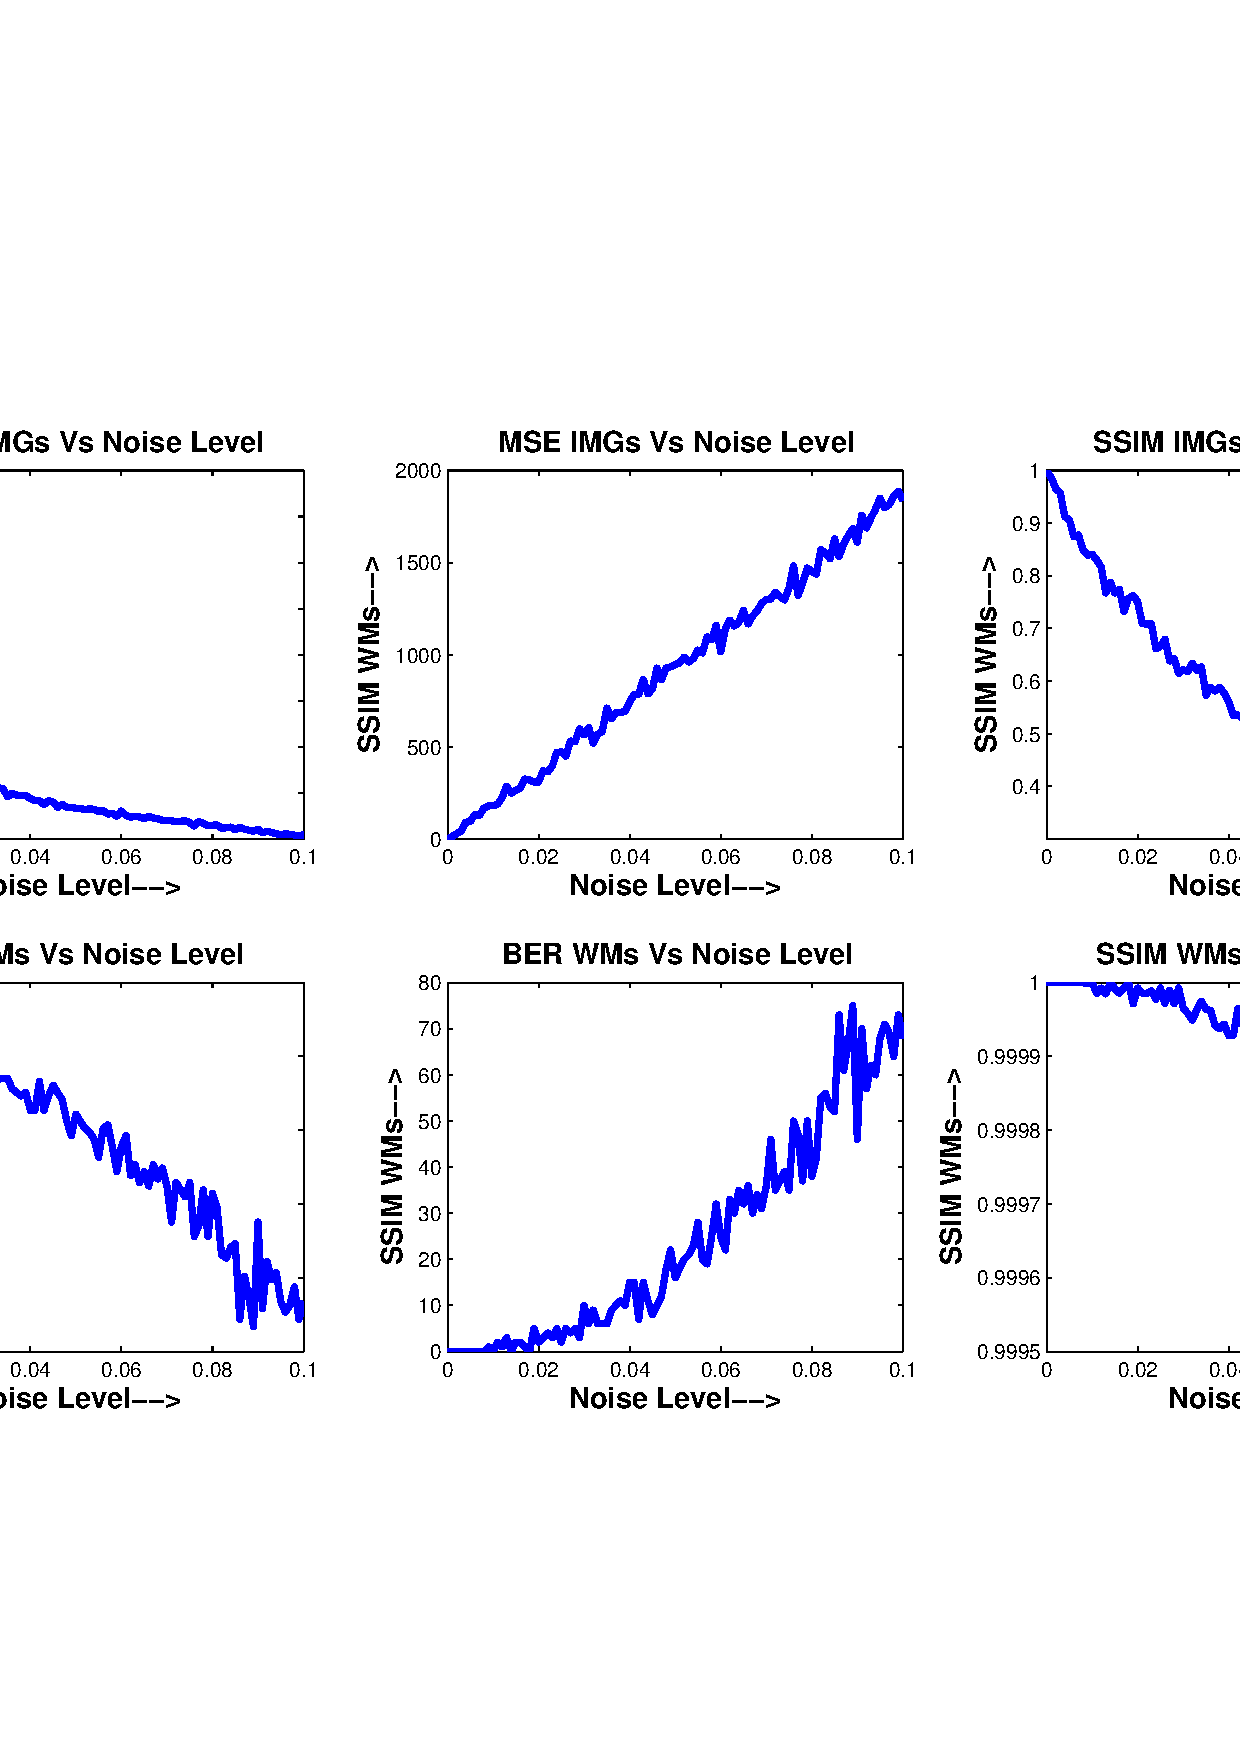
\includegraphics[width=1.0\linewidth]{./SaltPepper.png}
\caption{Salt \& Pepper Noise}
\label{WMSaltPepper}
\end{figure*}

	With the increase of salt \& pepper noise from 0 to 0.2 in steps of 0.002, PSNR is varied from 58.91 dB to 12.5 dB, MSE is varied from 0 to 3656, SSIM of watermarked image is varied from 1 to 0.2, NC is varied from 1 to 0.93, BER is varied from 0 to 0.07 and SSIM of watermark is varied from 1 to 0.998. From these results, it is clear that extracted watermark conveys the information with high NC and SSIM and with low BER.

\subsection{Gaussian Noise}
	By varying variance of additive white gaussian noise from 0 to 0.01 with mean 0, quality metrics like PSNR, MSE, SSIM are computed between Original image and watermarked image, $1^{st}$ row of Fig \ref{WMGaussian} represents these measurements. Similarly NC, BER, SSIM are computed between original watermark and extracted watermark, $2^{nd}$ row of Fig \ref{WMGaussian} represents these measurements. \\

	
\begin{figure*}
\centering
\includegraphics[width=1.0\linewidth]{./Gaussian.png}
\caption{Gaussian Noise}
\label{WMGaussian}
\end{figure*}

	With the increase of variance from 0 to 0.01 in steps of 0.0001 with mean 0, PSNR is varied from 58.91 dB to 20 dB, MSE is varied from 0 to 650, SSIM of watermarked image is varied from 1 to 0.48, NC is varied from 1 to 0.25, BER is varied from 0 to 0.76 and SSIM of watermark is varied from 1 to 0.928. From these results, it is clear that extracted watermark conveys the information with high NC and low BER and the performance is effective at lower variance levels of gaussian noise.

\subsection{Cropping Effect}
	With the variation of percentage of cropping from 0 to 100, quality measurements like PSNR, MSE, SSIM are computed between original image and watermarked image, $1^{st}$ row of Fig \ref{WMCrop} represents these measurements. Similarly NC, BER, SSIM are computed between original watermark and extracted watermark, $2^{nd}$ row of Fig \ref{WMCrop} represents these measurements. \\
	
\begin{figure*}
\centering
\includegraphics[width=1.0\linewidth]{./Cropping.png}
\caption{Cropping Effect}
\label{WMCrop}
\end{figure*}	
	
	With the increase of percentage of cropping from 0 to 100 in steps of 1, PSNR is varied from 58.91 dB to 6 dB,  SSIM of watermarked image is varied from 1 to 0, NC is varied from 1 to 0.1, BER is varied from 0 to 0.9 and SSIM of watermark is varied from 1 to 0.89. From these results, it is clear that extracted watermark conveys the information with higher SSIM factor and NC, BER are becoming poor as percentage of cropping is increased beyond 80. Reasonable watermark is extracted upto 80 percentage of cropping with NC, SSIM and BER of 0.42, 0.9425 and 0.52 respectively. 	
	
\subsection{JPEG Effect}
By varying quality factor from 0 to 100, quality measurements like PSNR, MSE, SSIM are computed between original image and watermarked image $1^{st}$ row of Fig \ref{WMJPeg} represents these measurements. Similarly NC, BER, SSIM are computed between original watermark and extracted watermark $2^{nd}$ row of Fig \ref{WMJPeg} represents these measurements. \\

\begin{figure*}
\centering
\includegraphics[width=1.0\linewidth]{./JpegQF.png}
\caption{JPEG Effect}
\label{WMJPeg}
\end{figure*}

With the increase of quality factor from 0 to 100 in steps of 1, PSNR is varied from 22 dB to 58.91 dB, MSE is varied from 410.28 to 0, SSIM of watermarked image is varied from 0.57 to 1, NC is varied from 0.32 to 1, BER is varied from 0.68 to 0 and SSIM of watermark is varied from 0.942 to 1. From these results, it is clear that extracted watermark conveys the information with high NC and low BER and the performance is effective towards higher quality factors of JPEG effect. The extracted watermark conveys the reasonable information effectively for the quality factors of 30 to 100 with NC of 0.52 to 1, BER of 0.56 to 1 and SSIM of 0.9734 to 1.


\subsection{Filtering}

Filtering like median, gaussian, averaging are applied on the watermarked imaged. Then, imperceptibility of the watermarked image and robustness of the extracted image are evaluated using the quality metrics. Quality metrics like PSNR, MSE, SSIM are computed between original image and watermarked image. Similarly NC, BER, SSIM are computed between original watermark and extracted watermark.\\
\textit {Median filtering} of $3$x$3$ is applied on the watermarked image. With median filtering PSNR of 35.11 dB is observed and extracted watermark shows NC of 0.82, BER of 0.16 having SSIM of 0.9950.
\textit {Gaussian filtering} of $3$x$3$ is applied on the watermarked image. PSNR of 31.26 dB is observed and extracted watermark shows NC of 0.76, BER of 0.2 having SSIM of 0.9921. 
\textit {Average filtering} of $3$x$3$ is applied on the watermarked image. PSNR of 30.12 dB is observed and extracted watermark shows NC of 0.7, BER of 0.212 having SSIM of 0.9889. 

 \subsection{Speckle noise}   
    Adding multiplicative noise to the watermarked image using the equation $J= I + n*I$. Where $I$ is watermarked image, $n$ is uniformly distributed random noise with mean 0 and variance V. By varying variance from 0 to 0.01, quality measurements like PSNR, MSE, SSIM are computed between original image and watermarked image, $1^{st}$ row of Fig \ref{WMSpeckle} represents these measurements. Similarly NC, BER, SSIM are computed between original watermark and extracted watermark, $2^{nd}$ row of Fig \ref{WMSpeckle} represents these measurements.\\
    
\begin{figure*}
\centering
\includegraphics[width=1.0\linewidth]{./Speckle.png}
\caption{Speckle Noise}
\label{WMSpeckle}
\end{figure*}  
        
    
    With the increase of variance from 0 to 0.01 in steps of 0.001, PSNR is varied from 58.91 dB to 26 dB, SSIM of watermarked image is varied from 1 to 0.72, NC is varied from 1 to 0.47, BER is varied from 0 to 0.55 and SSIM of watermark is varied from 1 to 0.96. From these results, it is clear that extracted watermark conveys the information in the presence of speckle noise.

 \subsection{Rotation Effect} 
 By varying rotation angle from -0.5 degree to 0.5 degree, quality measurements like PSNR, MSE, SSIM are computed between original image and watermarked image, $1^{st}$ row of Fig \ref{WMRot} represents these measurements. Similarly NC, BER, SSIM are computed between original watermark and extracted watermark, $2^{nd}$ row of Fig \ref{WMRot} represents these measurements.\\
 
\begin{figure*}
\centering
\includegraphics[width=1.0\linewidth]{./Rotation.png}
\caption{Rotation Effect}
\label{WMRot}
\end{figure*} 
 
 It is observed that, the proposed method works well only for smaller angles of rotations of the order $ < \pm { 0.4 } $ degree. With the order of rotation from 0 to 0.4 degree, PSNR is varied from 58.91 to 26, NC is varied from 1 to 0.47, BER is varied from 0 to 0.55 and SSIM of watermark is varied from 1 to 0.96. The method fails in conveying the message at higher degrees of rotations. 
 

\subsection{Comparison of watermarking with respect to different sized code book images } \label{SR}
The performance of proposed watermarking is compared with different sized code book images. Table \ref{TCPCBIM} gives comparison in the absence of noises. This shows that the effective retrieval of watermark with maximum NC and minimum BER is achieved even with smaller sized code book images, though such images have smaller PSNR. As our aim is to extract watermark reliably, so lower PSNR of the images can be relaxed and watermarking can be achieved with less computational complexity and less number of parameters.\\

\begin{table*}
\caption{Comparison of assessment metrics for different sized code book images without any noise}
\smallskip\noindent
\resizebox{\linewidth}{!}{%
\footnotesize
\label{TCPCBIM}
\begin{tabular}{@{}lcccc@{}}
\toprule
{\bf CB IMG SIZE (K)} & {\bf 128x128 (1)}           & {\bf 64x64 (2)}            & {\bf 32x32 (4)}            & {\bf 16x16 (8)}           \\ \midrule
{\bf PSNR(dB)}   & 58.911 	& 28.34  & 23.35  & 20.25     \\
{\bf NC}  & 1  	& 1 & 1 & 1                  \\
{\bf SSIM(WM)} & 1   		& 1 	 & 1	  & 1  	 \\
{\bf BER}   & 0 		& 0   	 & 0 	  &0    \\ 
{\bf SSIM(IMGS)}  & 0.9997  		& 0.8897 	 & 0.6867 	  & 0.4753 	 \\ 
\bottomrule
\end{tabular}}
\end{table*}


With the increase of percentage of cropping from 0 to 100, quality assessment metrics (PSNR, NC, BER, SSIM) are evaluated for four different sized code book images (K=1, 2, 4, 8). Fig \ref{CBCropping}(a) gives PSNR performance among four different sized code book images. PSNR decreases as percentage of cropping increases. Larger sized code book image shows higher PSNR values at lower percentage of cropping and PSNR values are same for all the four code book sized images as percentage of cropping reaches 100. Fig \ref{CBCropping}(b), Fig \ref{CBCropping}(c) and Fig \ref{CBCropping}(d) gives NC, BER and SSIM performance of four different sized code book images respectively. NC, BER, SSIM metrics are almost same for four different sized code book images.  \\

\begin{figure*}
\begin{tabular}{cc}
\includegraphics[width=2.75in]{./PSNRCP.png}&\includegraphics[width=2.75in]{./NCCP.png}\\
(a)  & (b) \\
\includegraphics[width=2.75in]{./BERCP.png}&\includegraphics[width=2.75in]{./SSIMCP.png}\\
(c)   & (d)
\end{tabular}
\caption{(a) PSNR Vs Percentage of Cropping, (b) NC Vs Percentage of Cropping,  (c) BER Vs Percentage of Cropping,  (d) SSIM Vs Percentage of Cropping }
\label{CBCropping}
\end{figure*} 

With the increase of gaussian noise variance from 0 to 0.001 with zero mean, quality assessment metrics (PSNR, NC, BER, SSIM) are evaluated for four different sized code book images (K=1, 2, 4, 8). Fig \ref{CBGaussian}(a) gives PSNR performance among four different sized code book images. PSNR decreases as the increase of variance. Larger sized code book image shows higher PSNR values and very small change in PSNR values is observed for all the four different sized code book images as variance is increased. Fig \ref{CBGaussian}(b), Fig \ref{CBGaussian}(c) and Fig \ref{CBGaussian}(d) gives NC, BER and SSIM performance of four different sized code book images respectively under gaussian noise. NC, BER, SSIM metrics are almost same for four different sized code book images.  \\

\begin{figure*}
\begin{tabular}{cc}
\includegraphics[width=2.75in]{./PSNRGS.png}&\includegraphics[width=2.75in]{./NCGS.png}\\
(a)  & (b) \\
\includegraphics[width=2.75in]{./BERGS.png}&\includegraphics[width=2.75in]{./SSIMGS.png}\\
(c)   & (d)
\end{tabular}
\caption{(a) PSNR Vs Variance, (b) NC Vs Variance,  (c) BER Vs Variance,  (d) SSIM Vs Variance }
\label{CBGaussian}
\end{figure*} 

With the increase of JPEG QF from 0 to 100, quality assessment metrics (PSNR, NC, BER, SSIM) are evaluated for four different sized code book images (K = 1, 2, 4, 8). Fig \ref{CBJPEG}(a) gives PSNR performance among four different sized code book images. PSNR increases with the increase of QF. Larger sized code book image shows higher PSNR values at higher QFs and PSNR values almost remains same for all the less sized  code book images. Fig \ref{CBJPEG}(b), Fig \ref{CBJPEG}(c) and Fig \ref{CBJPEG}(d) gives NC, BER and SSIM performance of four different sized code book images respectively under JPEG effect. Lesser is the size of code book image, better are the NC, BER, SSIM metrics. Up-sampled images (for K = 2, 4, 8) are more noisy compared to the image with K=1 case, so the impact of adding noise to images with K = 2, 4, 8 is less effective than that of the image with K = 1 case. \\

\begin{figure*}
\begin{tabular}{cc}
\includegraphics[width=2.75in]{./PSNRJG.png}&\includegraphics[width=2.75in]{./NCJG.png}\\
(a)  & (b) \\
\includegraphics[width=2.75in]{./BERJG.png}&\includegraphics[width=2.75in]{./SSIMJG.png}\\
(c)   & (d)
\end{tabular}
\caption{(a) PSNR Vs QF, (b) NC Vs QF,  (c) BER Vs QF,  (d) SSIM Vs QF }
\label{CBJPEG}
\end{figure*}

With the variation of rotation angle from -2 degree to 2 degree, quality assessment metrics (PSNR, NC, BER, SSIM) are evaluated for four different sized code book images (K=1, 2, 4, 8). Fig \ref{CBRotation}(a) gives PSNR performance among four different sized code book images. At lower angles of rotation i.e., from -0.4 degree to 0.4 degree only, watermark extraction with higher NC and lower BER is achieved. While, at higher angles of rotation, this method is not at all effective for extraction of watermark. Fig \ref{CBRotation}(b), Fig \ref{CBRotation}(c) and Fig \ref{CBRotation}(d) gives NC, BER and SSIM performance of four different sized code book images respectively. NC, BER, SSIM metrics shows that performance of extraction is better with the less sized code book image. Smaller is the size of the image lesser is the effect of rotation. \\

\begin{figure*}

\begin{tabular}{cc}
\includegraphics[width=2.75in]{./PSNRRO.png}&\includegraphics[width=2.75in]{./NCRO.png}\\
(a)  & (b) \\
\includegraphics[width=2.75in]{./BERRO.png}&\includegraphics[width=2.75in]{./SSIMRO.png}\\
(c)   & (d)
\end{tabular}
\caption{(a) PSNR Vs Angle, (b) NC Vs Angle,  (c) BER Vs Angle,  (d) SSIM Vs Angle }
\label{CBRotation}
\end{figure*}


With the increase of salt \& pepper noise from 0 to 0.3, quality assessment metrics (PSNR, NC, BER, SSIM) are evaluated for four different sized code book images (K=1, 2, 4, 8). Fig \ref{CBSaltPepper}(a) gives PSNR performance among four different sized code book images. PSNR decreases as salt \& pepper noise increases. Larger sized code book image shows higher PSNR values at lower noise levels and PSNR values are same for all the four code book sized images as salt \& pepper noise increases. Fig \ref{CBSaltPepper}(b), Fig \ref{CBSaltPepper}(c) and Fig \ref{CBSaltPepper}(d) gives NC , BER and SSIM performance of four different sized code book images respectively. Being extraction of watermark is the main objective, the relatively lower PSNR of the smaller sized code books does not restrict the usage of smaller code book sizes. This is mainly because NC, BER, SSIM metrics of watermark are almost same for four different sized code book images.

\begin{figure*}
\begin{tabular}{cc}
\includegraphics[width=2.75in]{./PSNRSP.png}&\includegraphics[width=2.75in]{./NCSP.png}\\
(a)  & (b) \\
\includegraphics[width=2.75in]{./BERSP.png}&\includegraphics[width=2.75in]{./SSIMSP.png}\\
(c)   & (d)
\end{tabular}
\caption{(a) PSNR Vs Noise, (b) NC Vs Noise,  (c) BER Vs Noise,  (d) SSIM Vs Noise }
\label{CBSaltPepper}

\end{figure*}

\subsection{Comparison with existing methods}

The proposed method is compared with that of existing techniques in the literature  \cite{P4}- \cite{P20}. The comparison of various quality assessment metrics with respect to attacks like JPEG,  median filtering, gaussian filtering, average filtering, salt \& pepper and cropping between proposed method (ACNNWM) and the method based on DWT level-2 decomposition, DCT and SVD (W2CS) as in \cite{P4} are given in Table \ref{MSGMP4}. The proposed method outperforms the method in \cite{P4} except at higher quality factors of JPEG compression effect having relatively lower NC.\\

\begin{table*}
\caption{Comparison with W2CS Method \cite{P4}  }
\smallskip\noindent
\resizebox{\linewidth}{!}{%
\footnotesize
\label{MSGMP4}
\begin{tabular}{@{}lcccc@{}}
\toprule
{\bf Method} & {}   &{ }      & {\bf W2CS \cite{P4}}            & {\bf ACNNWM }           \\ \midrule
{\bf No noise}		&{ }	& PSNR (dB) 	& 48.29 & \bf 58.91 \\
{ } 				& { } 	& NC 			&   1	& 1 \\
{\bf JPEG Comp} & QF:20 & PSNR 	& 25.39 & \bf 30.21 \\
{ } & { } & NC & 0.48 & \bf 0.56 \\ 
{ } &   QF:60 & PSNR 	& \bf 36.39 & 34.21 \\
{ } & { } & NC & \bf 0.90 & 0.64 \\ 
{ } &   QF:90 & PSNR 	& \bf 43.22 & 40.14 \\
{ } & { } & NC & \bf 0.94 & 0.72 \\ 
{\bf Median Filtering (3x3)}  &{ } & PSNR  	& 35.89 & \bf 36.42 \\
{ } & { } & NC & 0.21 & \bf 0.82 \\ 
{\bf Gaussian Filtering (3x3)}  &{ } & PSNR  	& \bf 37.44 &  31.27 \\
{ } & { } & NC & 0.49 & \bf 0.76 \\ 
{\bf Average Filtering (3x3)}  &{ } & PSNR  	& \bf 32.61 &  30.12 \\
{ } & { } & NC & 0.39 & \bf 0.72 \\ 
{\bf Salt $\&$ Pepper} & $\eta$:0.001 & PSNR 	& 46.14 & \bf 55.1  \\
{ } & { } & NC & 0.97 & \bf 1 \\ 
{ } & $\eta$:0.005 & PSNR 	& 43.04 & \bf 54.12  \\
{ } & { } & NC & 0.91 & \bf 1 \\ 
{\bf Cropping}    & 25$\%$	& NC 	&  0.81 & \bf 0.96 \\
%{\bf Gaussian Noise}   		& $\sigma$:10 & BER  	& 2.03 & \bf 0.9165 \\	
%{ } & $\sigma$:20 & BER & 15.16   & \bf 0.9163    \\ 
%{ } & $\sigma$:30 & BER & 28.69   & \bf 0.9165     \\
%
%{\bf Median Filtering (7x7)}  &{ } & BER  	& 7.1 & \bf 0.1626 \\
%{\bf Rotation (degree)} & $\theta$:-0.5 & BER  	& 36.86 & \bf 0.6008  \\
%{ } & $\theta$:0.5 & BER & 36.37   & \bf 0.5869     \\
\bottomrule
\end{tabular}}
\end{table*}

The comparison of various quality assessment metrics with respect to attacks like salt \& pepper, median filtering, gaussian filtering, average filtering,  JPEG and cropping between proposed method (ACNNWM) and the method based on level-1 decomposition of SWT and SVD (SW1S) as in \cite{P5} are given in Table \ref{WAMP5}. It is observed that the proposed method outperforms this SW1S method except at higher quality factors of JPEG compression effect having relatively lower NC.\\  


\begin{table*}
\caption{Comparison with SW1S Method \cite{P5} }
\smallskip\noindent
\resizebox{\linewidth}{!}{%
\footnotesize
\label{WAMP5}
\begin{tabular}{@{}lcccc@{}}
\toprule
{\bf Method} & {}   &{}      & {\bf SW1S \cite{P5}}            & {\bf ACNNWM }           \\ \midrule
{\bf No noise}    &{} 	& PSNR (dB) 	& 48.47 & \bf 58.91    \\
{ } 				& { } 	& NC 			&   1	& 1 \\
{ } 				& { } 	& BER 			&   0	& 0 \\
{\bf Salt $\&$ Pepper} & $\eta$:0.001 & PSNR 	& 43.53 & \bf 55.1  \\
{ } & { } & NC & 0.93 & \bf 1 \\ 
{ } 				& { } 	& BER 			&   0.12	& \bf 0 \\
{ } & $\eta$:0.005 & PSNR 	& 32.74 & \bf 54.12  \\
{ } & { } & NC & 0.81 & \bf 1 \\ 
{ } 				& { } 	& BER 			&   0.47	&  \bf 0 \\
{\bf Median Filtering (3x3)}  &{ } & PSNR  	& 32.12 & \bf 36.42 \\
{ } & { } & NC & 0.44 & \bf 0.82 \\ 
{\bf Gaussian Filtering (3x3)}  &{ } & PSNR  	& \bf 33.53 &  31.27 \\
{ } & { } & NC & 0.50 & \bf 0.76 \\ 
{\bf Average Filtering (3x3)}  &{ } & PSNR  	&  29.44 &  \bf 30.12 \\
{ } & { } & NC & 0.34 & \bf 0.72 \\ 
{\bf JPEG Comp} & QF:20 & PSNR 	& 25.39 & \bf 30.21 \\
{ } & { } & NC & 0.48 & \bf 0.56 \\ 
{ } &   QF:60 & PSNR 	& \bf 36.39 & 34.21 \\
{ } & { } & NC & \bf 0.90 & 0.64 \\ 
{ } &   QF:90 & PSNR 	& \bf 43.22 & 40.14 \\
{ } & { } & NC & \bf 0.94 & 0.72 \\ 
{\bf Cropping}    & 25$\%$	& NC 	&  0.64 & \bf 0.96 \\
{ } & { } & BER & 0.71 & \bf 0.05\\
\bottomrule
\end{tabular}}
\end{table*}

The comparison of various quality assessment metrics with respect to attacks like median filtering, gaussian filtering, average filtering, salt \& pepper, JPEG compression and cropping between proposed method (ACNNWM) and the method based on level-1 decomposition of DWT along with DCT (W1C) as in \cite{P6} are given in Table \ref{DCTWMP6}. It is observed that the proposed method outperforms this W1C method in all cases except in case of higher quality JPEG effect where the proposed method is giving slightly less correlation value with allowable information content perceived by human eye after extraction.\\


\begin{table*}
\caption{Comparison with W1C Method as in \cite{P6}}
\smallskip\noindent
\resizebox{\linewidth}{!}{%
\footnotesize
\label{DCTWMP6}
\begin{tabular}{@{}lcccc@{}}
\toprule
{\bf Method} & {}   & {}       & {\bf W1C\cite{P6}}            & {\bf ACNNWM }           \\ \midrule
{\bf No noise}		&{ }	& PSNR (dB) 	& 51.45 & \bf 58.91 \\
{ } 				& { } 	& NC 			&   1	& 1 \\
{\bf Median Filtering (3x3)}  &{ } & PSNR  	& \bf 36.71 &  36.42 \\
{ } & { } & NC & 0.78 & \bf 0.82 \\ 
{\bf Gaussian Filtering (3x3)}  &{ } & PSNR  	& \bf 33.99 &  31.27 \\
{ } & { } & NC & 0.68 & \bf 0.76 \\ 
{\bf Average Filtering (3x3)}  &{ } & PSNR  	&  25.51 &  \bf 30.12 \\
{ } & { } & NC & 0.26 & \bf 0.72 \\ 
{\bf Salt $\&$ Pepper} & $\eta$:0.001 & PSNR 	& 34.61 & \bf 55.1  \\
{ } & { } & NC & 0.96 & \bf 1 \\ 
{ } & $\eta$:0.005 & PSNR 	& 31.66 & \bf 54.12  \\
{ } & { } & NC & 0.92 & \bf 1 \\ 
{\bf JPEG Comp} & QF:20 & PSNR 	& 26.54 & \bf 30.21 \\
{ } & { } & NC & 0.51 & \bf 0.56 \\ 
{ } &   QF:90 & PSNR 	& \bf 45.48 & 40.14 \\
{ } & { } & NC & \bf 0.91 & 0.72 \\ 
{\bf Cropping}    & 25$\%$	& NC 	&  0.71 & \bf 0.96 \\
\bottomrule
\end{tabular}}
\end{table*}


The comparison of various quality assessment metrics with respect to attacks like median filtering, gaussian filtering, average filtering, salt \& pepper, JPEG compression and cropping between proposed method (ACNNWM) and the method based on level-1 decomposition of DWT along with SVD LU decomposition (W1SLU) as in \cite{P7} are given in Table \ref{MBWDMP7}. The proposed method outperforms this W1SLU method in all cases and in cases like average filtering , higher quality JPEG effects the performances of these methods are almost similar.\\


\begin{table*}
\caption{Comparison with W1SLU Method as in \cite{P7} }
\smallskip\noindent
\resizebox{\linewidth}{!}{%
\footnotesize
\label{MBWDMP7}
\begin{tabular}{@{}lcccc@{}}
\toprule
{\bf Method} & {}  &{}       & {\bf W1SLU\cite{P7}}            & {\bf ACNNWM }           \\ \midrule
{\bf No noise}		&{ }	& PSNR (dB) 	& 34.33 & \bf 58.91 \\
{ } 				& { } 	& NC 			&   1	& 1 \\
{\bf Median Filtering (3x3)}  &{ } & PSNR  	& 32.11 &  \bf 36.42 \\
{ } & { } & NC & 0.62 & \bf 0.82 \\ 
{\bf Gaussian Filtering (3x3)}  &{ } & PSNR  	&  30.28 & \bf 31.27 \\
{ } & { } & NC & 0.69 & \bf 0.76 \\ 
{\bf Average Filtering (3x3)}  &{ } & PSNR  	& \bf 30.51 &   30.12 \\
{ } & { } & NC & \bf 0.86 &  0.72 \\ 
{\bf Salt $\&$ Pepper} & $\eta$:0.001 & PSNR 	& 26.2 & \bf 55.1  \\
{ } & { } & NC & 0.94 & \bf 1 \\ 
{ } & $\eta$:0.005 & PSNR 	& 22.43 & \bf 54.12  \\
{ } & { } & NC & 0.91 & \bf 1 \\ 
{\bf JPEG Comp} & QF:20 & PSNR 	& 16.34 & \bf 30.21 \\
{ } & { } & NC & 0.32 & \bf 0.56 \\ 
{ } &   QF:90 & PSNR 	&  30.26 & \bf 40.14 \\
{ } & { } & NC & \bf 0.74 & 0.72 \\ 
{\bf Cropping}    & 25$\%$	& NC 	&  0.86 & \bf 0.96 \\

\bottomrule
\end{tabular}}
\end{table*}


The comparison in case of  median filtering, gaussian filtering, average filtering, salt \& pepper, JPEG compression and cropping of various quality assessment metrics between proposed method (ACNNWM) and the method based on DCT and level-3 decomposition of DWT (CW3) as in \cite{P20} are given in Table \ref{CW3P20}. The proposed method outperforms this CW3 method in all cases and the performance is comparable at higher quality JPEG effects.\\

\begin{table*}
\caption{Comparison with CW3 Method as in \cite{P20} }
\smallskip\noindent
\resizebox{\linewidth}{!}{%
\footnotesize
\label{CW3P20}
\begin{tabular}{@{}lcccc@{}}
\toprule
{\bf Method} 			& {}	& {}      	& {\bf CW3\cite{P20}}	& {\bf ACNNWM }           \\ \midrule
{\bf No noise}			&{ }	& PSNR (dB) & 56.74 				& \bf 58.91 \\
{ } 					& { } 	& NC 		&   1					& 1 \\
{\bf Median Filtering (3x3)}  &{ } & PSNR  	& 34.54 				&  \bf 36.42 \\
{ } 					& { } 	& NC 		& 0.80				 	& \bf 0.82 \\ 
{\bf Gaussian Filtering (3x3)}  &{ } & PSNR &  30.68				& \bf 31.27 \\
{ } 					& { } 	& NC 		& 0.72 					& \bf 0.76 \\ 
{\bf Average Filtering (3x3)}  &{ } & PSNR  &  28.81 				&   \bf 30.12 \\
{ } 					& { } 	& NC 		& 0.67 					&   \bf 0.72 \\ 
{\bf Salt $\&$ Pepper} & $\eta$:0.001 & PSNR & 44.24				& \bf 55.1  \\
{ } 					& { } 	& NC 		& 0.96 					& \bf 1 \\ 
{ } 					& $\eta$:0.005 & PSNR & 40.18 				& \bf 54.12  \\
{ } 					& { } 	& NC 		& 0.93 					& \bf 1 \\ 
{\bf JPEG Comp} 		& QF:20 & PSNR 		& 28.94			& \bf 30.21 \\
{ } 					& { } 	& NC 		& 0.56					& \bf 0.56 \\ 
{ } 					& QF:90 & PSNR 		&  37.86				& \bf 40.14 \\
{ } 					& { } 	& NC 		& \bf 0.84 				& 0.72 \\ 
{\bf Cropping}    		& 25$\%$& NC 		&  0.89 				& \bf 0.96 \\
\bottomrule
\end{tabular}}
\end{table*}

The overall performance of the proposed method with respect to all other methods is shown in Table \ref{TotMethods} where the performance rank of the proposed method is given in the braces of the last column.
\begin{table*}
\caption{Comparison with different methods}
\smallskip\noindent
\resizebox{\linewidth}{!}{%
\footnotesize
\label{TotMethods}
\begin{tabular}{@{}lcccccccccc@{}}
\toprule
{\bf Method} 			& {}	& {}    &{\bf W2CS \cite{P4}} & {\bf SW1S \cite{P5}}  &{\bf W1C \cite{P6}}     & {\bf W1SLU \cite{P7}}  & {\bf CW3 \cite{P20}}	&{\bf  1PW1 \cite{P21}} &{\bf SCD \cite{P22}}& {\bf ACNNWM } \\
{} 			& {}	& {}    &{} & {}  &{}     & {}  & {}	&{} &{}& {(Rank) }                   \\ \midrule
{\bf No noise}			&{ }	& PSNR (dB) &{48.29}  & {48.47} & {51.45} & {34.33}& 56.74 		&{35.6} &{47}		& \bf 58.91(1) \\
{ } 					& { } 	& NC 		&{1.00}      & {1.00}     & {1.00} & {1.00}&   1.00 &{0.99}	 &{0.98}				& 1.00(1) \\
{\bf Median Filtering (3x3)}  &{ } & PSNR  	&{35.89}  & {32.12} & {\bf 36.71} & {32.11}& 34.54  &{32.44} &{30.18}		&   36.42(2) \\
{ } 					& { } 	& NC 		&{0.21}   & {0.44}  & {0.78} & {0.62}& 0.80			&{0.6} &{0.23}	 	& \bf 0.82(1) \\ 
{\bf Gaussian Filtering (3x3)}  &{ } & PSNR &{\bf 37.44}  & {33.53} & {33.99} & {30.28}&  30.68	&{30.12}	&{30.16}		& 31.27(4)\\
{ } 					& { } 	& NC 		&{0.49}   & {0.50}   & {0.68} & {0.69}& 0.72 		&{0.61}	&{0.43}		& \bf 0.76(1) \\ 
{\bf Average Filtering (3x3)}  &{ } & PSNR &{\bf 32.61}   & {29.44} & {25.51}  & {30.51}&  28.81 &{29.68}	&{29.6}			&   30.12(3) \\
{ } 					& { } 	& NC 		&{0.39}   & {0.34}  & {0.26}  & {\bf 0.86}& 0.67 	&{0.72} &{0.4}				&   0.72(2) \\ 
{\bf Salt $\&$ Pepper} & $\eta$:0.001 & PSNR &{46.14} & {43.53} & {34.61} & {26.2}& 44.24		&{31.44} &{44.22}		& \bf 55.10(1)  \\
{ } 					& { } 	& NC 		&{0.97}   & {0.93}  & {0.96} & {0.94}& 0.96 		&{0.97} &{0.95}			& \bf 1.00(1)\\ 
{ } 					& $\eta$:0.005 & PSNR &{43.04}& {32.74} & {31.66} & {22.43}& 40.18 		&{29.1} &{41.72}		& \bf 54.12(1)  \\
{ } 					& { } 	& NC 		&{0.91}   & {0.81}  & {0.92} & {0.91}& 0.93 		&{0.95} &{0.91}			& \bf 1.00(1) \\ 
{\bf JPEG Comp} 		& QF:20 & PSNR 		&{25.39}  & {25.38} & {26.54} & {16.34}& 28.94		&{22.4}	&{23.8} & \bf 30.21(1) \\
{ } 					& { } 	& NC 		&{0.48}   & {0.44}  & {0.51} & {0.32}& 0.56			&{0.42}	&{0.5}	& \bf 0.56 (1)\\ 
{ } 					& QF:90 & PSNR 		&{ 43.22}  & {42.1} & {\bf 45.48} & {30.26}&  37.86	&{31.55}	&{42.6}		& 40.14(5) \\
{ } 					& { } 	& NC 		&{\bf 0.94}   & {0.9}  & {0.91} & {0.74}&  0.84 	&{0.8}	&{0.9}		& 0.72(7) \\ 
{\bf Cropping}    		& 25$\%$& NC 		&{0.81}   & {0.64}  & {0.71} & {0.86}&  0.89 		&{0.91} &{0.9}		& \bf 0.96(1) \\
\bottomrule
\end{tabular}}
\end{table*}

From the comparisons with different non blind watermarking approaches, it is concluded that the proposed CNN based non blind watermarking technique is robust to different attacks, filtering operations, compressions and produces on par results at higher quality JPEG effects in terms NC, BER \\
 
 The performance of the proposed method (ACNNWM) is poor under following cases: $i)$ At higher variance of the gaussian noise; $ii)$ At lower quality factors under JPEG effect; $iii)$  At higher rotational attacks $>\pm$ 0.5 degree.


 

